\documentclass[a4paper]{article}
\usepackage[margin=1in]{geometry}
\usepackage[english]{babel}
\usepackage[utf8]{inputenc}
\usepackage{amsmath}
\usepackage{graphicx}
\usepackage{amssymb}
\usepackage{amsthm}
\usepackage{tikz-cd}
\usepackage{mathrsfs}
\usepackage[colorinlistoftodos]{todonotes}
\usepackage{enumitem}
\usepackage{yfonts}
\usepackage{dsfont}
\usepackage{mathtools}
\usepackage{hyperref}
\usepackage{pgfplots}

\pgfplotsset{compat=1.18}
\usetikzlibrary{arrows.meta, calc}
\DeclarePairedDelimiter\ceil{\lceil}{\rceil}
\DeclarePairedDelimiter\floor{\lfloor}{\rfloor}

\title{Convex Optimization Notes}

\author{Wilson Pan}

\date{\today}

\newtheorem{thm}{Theorem}[section]
\newtheorem{lem}[thm]{Lemma}
\newtheorem{defn}[thm]{Definition}
\newtheorem{eg}[thm]{Example}
\newtheorem{ex}[thm]{Exercise}
\newtheorem{conj}[thm]{Conjecture}
\newtheorem{cor}[thm]{Corollary}
\newtheorem{claim}[thm]{Claim}
\newtheorem{rmk}[thm]{Remark}
\newtheorem{rec}[thm]{Recall}

\newcommand{\ie}{\emph{i.e.}\ }
\newcommand{\cf}{\emph{cf.}\ }
\newcommand{\into}{\hookrightarrow}
\newcommand{\dirac}{\slashed{\partial}}
\newcommand{\R}{\mathbb{R}}
\newcommand{\C}{\mathbb{C}}
\newcommand{\Z}{\mathbb{Z}}
\newcommand{\N}{\mathbb{N}}
\newcommand{\Q}{\mathbb{Q}}
\newcommand{\LieT}{\mathfrak{t}}
\newcommand{\T}{\mathbb{T}}
\newcommand{\A}{\mathds{A}}
\newcommand{\HG}{\mathcal{H}}
\newcommand{\F}{\mathbb{F}}
\newcommand{\poly}[2]{\text{Poly}_{#1}(#2)}
\newcommand{\gen}[1]{\langle #1 \rangle}
\newcommand{\Hom}{\text{Hom}}
\newcommand{\norm}[1]{\lVert #1\rVert}
\newcommand{\aff}{\mathrm{Aff}}

\begin{document}
\maketitle
\tableofcontents
\newpage

\section{Jan 13}
\begin{defn}
    An \textbf{optimization problem} is defined as
    \[
        \min_{x \in \mathcal{C}} f_0(x) \quad \text{where} \quad \forall i \in [m],\; f_i(x) \leq b_i
    \]
    where $\mathcal{C}$ is the constraint set and $f_0\colon \mathcal{C} \to \R$.
\end{defn}

\begin{defn}
    The \textbf{standard form} of an optimization problem is
    \[
        \min_{x \in \mathcal{D}} f_0(x) \quad \text{subject to} \quad
        \forall i \in [m],\ f_i(x) \leq 0; \quad \forall j \in [p],\ h_j(x) = 0
    \]
    where $x \in \mathrm{dom}(f_i) \cap \mathrm{dom}(h_j) =: \mathcal{D}$.
    \\
    $f_0$ is termed the \emph{objective function}, and $x$ is the optimization variable.\\
    $f_i$ and $h_j$ are constraint functions.
\end{defn}

\begin{defn}
    A \textbf{feasible solution} is any $x \in \mathcal{D}$ that satisfies all the constraints.
\end{defn}

\begin{defn}
    The \textbf{optimal solution} is $x^* \in \arg\min_{x \in \mathcal{D}} f_0(x)$.
\end{defn}

\begin{rmk}
    If no feasible solution exists, we define $\min_{x \in \mathcal{C}} f(x) = +\infty$ and, similarly, $\max_{x \in \mathcal{C}} f(x) = -\infty$.
\end{rmk}

\newpage
\section{Jan 15}
\begin{defn}
    A set $C$ is \textbf{convex} if $\forall x_1, x_2 \in C$ and $\forall \theta \in [0, 1]$, we have $\theta x_1 + (1-\theta)x_2 \in C$.
\end{defn}

\begin{defn}
    A function $f\colon \mathcal{X} \to \R$ is \textbf{convex} if for all $x_1, x_2 \in \mathcal{X}$ and $\theta \in [0, 1]$,
    \begin{align*}
        f(\theta x_1 + (1-\theta)x_2) \leq \theta f(x_1) + (1-\theta)f(x_2) \tag{*}
    \end{align*}
\end{defn}

\begin{rmk}
    Convex functions are differentiable almost everywhere.
\end{rmk}

\begin{thm}
    If $f$ is both convex and concave, then $f$ is affine (i.e., linear plus constant).
\end{thm}

\begin{defn}
    $f$ is \textbf{strictly convex} if $(*)$ holds with strict inequality $\;<$ whenever $x_1 \neq x_2$ and $\theta \in (0, 1)$.
\end{defn}

\begin{defn}
    A \textbf{convex optimization problem} is one where $f_0$, $f_i$, and $\mathcal{C}$ are convex, and $h_j$ are affine/linear. That is,
    \[
        \min_{x \in \mathcal{C}} f_0(x)
        \quad\text{such that}\quad
        f_i(x) \leq 0\;\; \forall i \in [m], \quad h_j(x) = 0\;\; \forall j \in [p]
    \]
\end{defn}

\begin{thm}
    The set of feasible solutions in Definition 2.6 is convex.
\end{thm}

\begin{thm}
    $x^*$ is a \textbf{local minimizer} if there exists $\epsilon > 0$ such that for all $y$ with $\norm{x^* - y} \leq \epsilon$,
    \[
        f(x^*) \leq f(y)
    \]
\end{thm}

\begin{thm}
    $x^*$ is a \textbf{local maximizer} if there exists $\epsilon > 0$ such that for all $y$ with $\norm{x^* - y} \leq \epsilon$,
    \[
        f(x^*) \geq f(y)
    \]
\end{thm}

\begin{thm}
    For any convex optimization problem, every local minimum is a global minimum.
    \begin{proof}
        Suppose $\hat{x}$ is a local minimizer not equal to global minimizer $x^*$. Take $\epsilon$ as any witness to $\hat{x}$ being a local minimum. Let
        \[
            y = \frac{\epsilon}{\norm{\hat{x} - x^*}} x^* + \left(1 - \frac{\epsilon}{\norm{\hat{x} - x^*}}\right) \hat{x}
        \]
        Note: $\norm{\hat{x} - x^*} \leq \epsilon$, otherwise $\hat{x}$ is not a local minimizer in that neighborhood.
        \[
            y - \hat{x} = \frac{\epsilon (x^* - \hat{x})}{\norm{x^* - \hat{x}}} \quad;\quad \norm{y - \hat{x}} = \epsilon
        \]
        Since $f$ is convex,
        \[
            f(y) \leq \frac{\epsilon}{\norm{\hat{x} - x^*}} f(x^*) + \left(1-\frac{\epsilon}{\norm{\hat{x} - x^*}}\right) f(\hat{x}) < f(\hat{x})
        \]
        Thus, a contradiction.
    \end{proof}
\end{thm}

\newpage
\section{Jan 20}
\begin{defn}
    A \textbf{convex combination} of $x_1, x_2$ is $\theta_1 x_1 + \theta_2 x_2$ where $\theta_1, \theta_2 \geq 0$ and $\theta_1 + \theta_2 = 1$.
\end{defn}

\begin{defn}
    An \textbf{affine combination} of $x_1, x_2$ is $\theta_1 x_1 + \theta_2 x_2$ where $\theta_1 + \theta_2 = 1$.
\end{defn}

\begin{defn}
    A \textbf{linear combination} of $x_1, x_2$ is $\theta_1 x_1 + \theta_2 x_2$ where $\theta_1, \theta_2 \in \R$.
\end{defn}

\begin{defn}
    A \textbf{conic combination} of $x_1, x_2$ is $\theta_1 x_1 + \theta_2 x_2$ where $\theta_1, \theta_2 \geq 0$.
\end{defn}

\begin{defn}
    Given a set $C$, the \textbf{convex hull} of $C$ is
    \[
        \mathrm{conv}(C) = \left\{ \sum_{i=1}^k \theta_i x_i \;\middle|\; x_i \in C,\, \theta_i \in [0,1],\, \sum_{i=1}^k \theta_i = 1 \right\}
    \]
\end{defn}

\begin{rmk}
    The following are true:
    \begin{enumerate}
        \item $C \subseteq \mathrm{conv}(C)$
        \item $\mathrm{conv}(C)$ is convex
        \item It is the smallest convex set containing $C$
        \item If a convex set $S \supseteq C$ then $S \supseteq \mathrm{conv}(C)$
    \end{enumerate}
\end{rmk}

\begin{thm}
    Any closed convex set can be written as $\overline{\mathrm{conv}}(C)$ for some set $C$.
\end{thm}

\begin{defn}
    The \textbf{relative interior} of $C$ is defined as
    \[
        \mathrm{relint}(C) = \left\{ x \in C : \exists \epsilon > 0,\ B(x, \epsilon) \cap \aff(C) \subseteq C \right\}
    \]
\end{defn}

\begin{defn}
    $C$ is a \textbf{cone} if $\alpha x \in C$ whenever $x \in C$ and $\alpha \geq 0$.
\end{defn}

\begin{defn}
    Given a set $C$, the \textbf{conic hull} of $C$ is
    \[
        \mathrm{conic}(C) = \left\{ \sum_{i=1}^k \theta_i x_i : x_i \in C,\ \theta_i \geq 0 \right\}
    \]
\end{defn}

\begin{thm}
    The conic hull of $C$ is the smallest convex cone containing $C$.
\end{thm}

\begin{defn}
    The \textbf{$\ell_p$ norm} is defined as 
    \[
        \norm{x}_p = \left( \sum_{i=1}^d |x_i|^p \right)^{1/p}
    \]
\end{defn}

\begin{rmk}
    The following are true:
    \begin{enumerate}
        \item For $p \in (0,1)$: $\norm{x}_p$ is not a convex function
        \item For $p \geq 1$: $\norm{x}_p$ is convex
        \item For $p > 1$: $\norm{x}_p$ is strictly convex
    \end{enumerate}
\end{rmk}

\begin{eg}
    Examples of convex sets:
    \begin{enumerate}
        \item Hyperplane: $\{ x : a^T x = b \}$
        \item Halfspace: $\{ x : a^T x \leq b \}$
        \item Polyhedron: $\{ x \in \R^d : Ax \leq b,\; Cx = d \}$
        \item Polytope: a bounded polyhedron.
    \end{enumerate}
\end{eg}

\begin{thm}
    A set $S$ is \textbf{strictly convex} if for all $x_1 \neq x_2$ and $\theta \in (0, 1)$, $\theta x_1 + (1-\theta) x_2 \in \mathrm{int}(S)$.
\end{thm}

\begin{defn}
    The \textbf{normal cone} is defined to be
    \[
        N_C(x) = \{ g : g^T(y - x) \leq 0,\ \forall y \in C \}
    \]
\end{defn}

\begin{rmk}
    If $x \in \mathrm{int}(C)$ then $N_C(x) = \{0\}$.
\end{rmk}

\begin{thm}
    If $f$ is differentiable, then $x^*$ is optimal if and only if $-\nabla f(x^*) \in N_C(x^*)$.
\end{thm}

\newpage
\section{Jan 22}
\begin{thm}
    If $f$ is convex and differentiable, and $C$ is a convex set, then any optimal solution $x^*$ to $\min_{x \in C} f(x)$ must satisfy $-\nabla f(x^*) \in N_C(x^*)$.
\end{thm}

\begin{thm}
    The set of optimal solutions to a convex optimization problem is a convex set.
\end{thm}

\begin{defn}
    If $C$ is convex then
    \begin{enumerate}
        \item \textbf{Translation:} $C+a = \{ x : x-a \in C \}$
        \item \textbf{Scaling:} $\alpha C = \{ x : \frac{x}{\alpha} \in C \}$
        \item \textbf{Intersection:} If $\{C_\alpha\}_{\alpha \in A}$ is a collection of convex sets, then $\bigcap_{\alpha \in A} C_\alpha$ is convex.
    \end{enumerate}
\end{defn}

\begin{thm}
    The following are true:
    \begin{enumerate}
        \item If $C \subseteq \R^n$ is convex, $A \in \R^{m \times n}$ and $b \in \R^m$, then $AC + b = \{ Ax + b : x \in C \}$ is a convex set.
        \item If $f(x) = Ax + b$, then $f^{-1}(C)$ is convex.
        \item $C_1 + C_2 = \{ x + y : x \in C_1,\, y \in C_2 \}$ is convex.
        \item If $C_1 \subseteq \R^m,\, C_2 \subseteq \R^n$ then $C_1 \times C_2 = \{ (x, y) \in \R^{m+n} : x \in C_1,\, y \in C_2 \}$ is convex.
        \item For any $C \subseteq \R^n \times \R_{>0}^m$, define
        \[
            P(C) = \left\{ \left( \frac{x_1}{t}, \ldots, \frac{x_n}{t} \right) : (x_1, \ldots, x_n, t) \in C \right\}
        \]
        If $C$ is convex, so are $P(C)$ and $P^{-1}(C)$.
    \end{enumerate}
\end{thm}

\begin{defn}
    \[
        \mathrm{epi}(f) = \{ (x, t) : x \in \mathrm{dom}(f),\, t \geq f(x) \}
    \]
\end{defn}

\begin{defn}
    \textbf{First Order Definition of Convexity:} If $f$ is differentiable, then $f$ is convex if and only if for all $x, y \in \mathrm{dom}(f)$,
    \[
        f(y) \geq f(x) + \nabla f(x)^T (y - x)
    \]
    \begin{figure}[h]
        \centering
        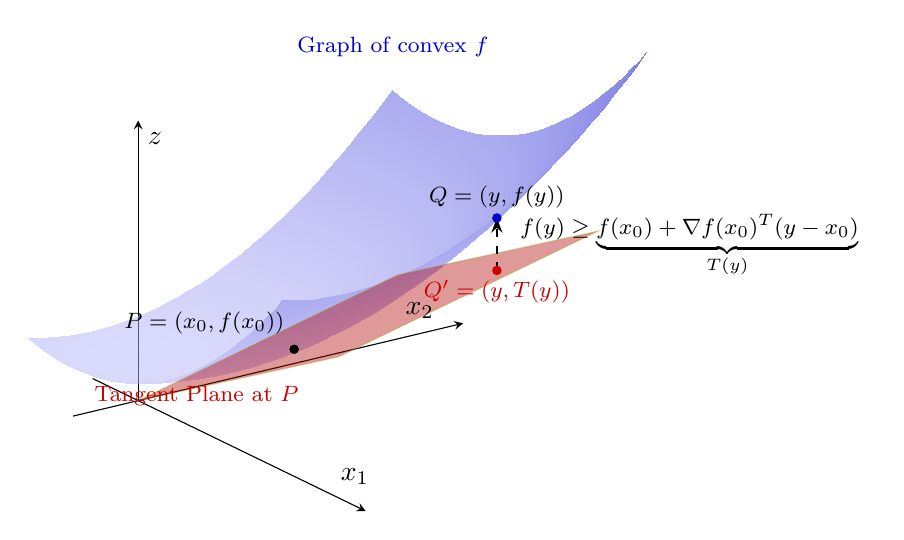
\begin{tikzpicture}
            \begin{axis}[
                view={55}{30},
                axis lines=middle,
                xlabel={$x_1$}, ylabel={$x_2$}, zlabel={$z$},
                xmin=-0.5, xmax=2.5,
                ymin=-0.5, ymax=2.5,
                zmin=0, zmax=3.5,
                xtick=\empty, ytick=\empty, ztick=\empty,
                domain=-0.5:2.3,
                y domain=-0.5:2.3,
                samples=35,
                clip=false,
                width=10cm, height=8cm
            ]
                \def\fval(#1,#2) {0.4*(#1)^2 + 0.4*(#2)^2 + 0.5}
                \def\tval(#1,#2) {0.8*(#1) + 0.4*(#2)}
                \addplot3[
                    surf,
                    opacity=0.5,
                    shader=interp,
                    colormap={bluewhite}{color(0cm)=(white!80!blue); color(1cm)=(blue!80!black)},
                    z buffer=sort
                ] { \fval(x,y) };
                \addplot3[
                    surf,
                    opacity=0.4,
                    color=red!70!black,
                    z buffer=sort,
                    samples=2,
                    domain=0:2.2,
                    y domain=0:2.0
                ] { \tval(x,y) };
                \coordinate (P) at (1, 0.5, 1.0);
                \addplot3[mark=*, mark size=1.5pt, color=black] coordinates {(1, 0.5, 1.0)};
                \node[font=\footnotesize, above left, yshift=2pt] at (P) {$P=(x_0, f(x_0))$};
                \coordinate (Q) at (1.8, 1.5, 2.696);
                \addplot3[mark=*, mark size=1.5pt, color=blue!80!black] coordinates {(1.8, 1.5, 2.696)};
                \node[font=\footnotesize, above] at (Q) {$Q=(y, f(y))$};
                \coordinate (Qprime) at (1.8, 1.5, 2.04);
                \addplot3[mark=*, mark size=1.5pt, color=red!80!black] coordinates {(1.8, 1.5, 2.04)};
                \node[font=\footnotesize, below, color=red!80!black] at (Qprime) {$Q'=(y, T(y))$};
                \draw[dashed, thick, -{Stealth[scale=0.8]}, color=black] (Qprime) -- (Q);
                \node[font=\footnotesize, right, align=left, xshift=5pt] at (1.8, 1.5, 2.35) {
                    $f(y) \ge \underbrace{f(x_0) + \nabla f(x_0)^T(y - x_0)}_{T(y)}$
                };
                \node[font=\footnotesize, blue!80!black] at (-0.2, 2.1, 3.5) {Graph of convex $f$};
                \node[font=\footnotesize, red!80!black] at (0.5, 0.1, 0.3) {Tangent Plane at $P$};
            \end{axis}
        \end{tikzpicture}
        \caption{First Order Definition of Convexity}
    \end{figure}\\
    \noindent \textbf{Second Order Definition of Convexity:} If $f$ is twice differentiable, then $f$ is convex if and only if $\nabla^2 f(x) \succeq 0$.
\end{defn}

\begin{defn}
    We say $A \succeq B$ if $A - B$ is positive semi-definite. This is equivalent to
    \[
        a^T \nabla^2 f(x) a \geq 0 \quad \text{for all}\ a \in \R^d
    \]
\end{defn}

\begin{defn}
    The \textbf{subdifferential} is
    \[
        \partial f(x) = \left\{ g : f(y) \geq f(x) + g^T (y-x),\ \forall y \in C \right\}
    \]
    Any such $g \in \partial f(x)$ is called a \textbf{subgradient}.\\
    If $f$ is differentiable at $x$ then $\partial f(x) = \{ \nabla f(x) \}$.
\end{defn}
\begin{thm}
    $f$ is convex if and only if $\partial f$ is non-empty. 
\end{thm}

\newpage
\section{Jan 27}
\begin{defn}
    Gradient Monotonicity: If $f$ is differentiable, then $f$ is convex if and only if $\nabla f(x)$ is monotone. So we can conclude \[
    (\nabla f(x) - \nabla f(y))^T(x-y)\geq 0 \iff f \text{ is convex}
    .\] 
\end{defn}
\begin{thm}
    For a $A\in \R^{m\times n}$ we can decompose \[
        A=U \sum V^t
    .\] where $U\in \R^{m \times k}$ with orthonormal column, $\sigma\in \R^{k\times k}$ is a diagonal matrix with non-negative entries, and $V\in \R^{n\times k}$ with orthonormal column.
\end{thm}
\begin{defn}
    $(u_i,v_i,\sigma_i)$ form a s.v. triplet if $Av_i=\sigma_i u_i$ and $A^T u_i=\sigma_i v_i$\\
    $||u_i||=||v_i||=1$ and $\sigma_i\geq 0$
\end{defn}
\begin{thm}
    For any $A\in \R^{n\times n}$ then $A^TA$ is always positive semi definite
    \begin{proof}
        We can write $A=V \sum U$ then $A^TA=V\sum U^T U \sum V^T=V \sum^2 V^T$
    \end{proof}
\end{thm}
\begin{defn}
    Spectral Radius: $\max_i\{|\lambda_i| : \lambda_i \in \Lambda(A)\}=\rho(A)$
\end{defn}
\begin{defn}
    The norm must satisfy the following properties:
    \begin{enumerate}
        \item $||A||\geq 0$
        \item $||\alpha A||= |\alpha|||A||$
        \item $||A||=0$ if and only if $A=0$
        \item $||A+A'||\leq ||A||+||A'||$
    \end{enumerate}
\end{defn}
\begin{defn}
    Operator/Spectral Norm: \[
    ||A||_{\text{op}}=||A||_2=\max_{||x||=1}||Ax||_2
    .\] 
\end{defn}
\begin{defn}
    Frobenius Norm: \[
    ||A||_F=\sqrt{\sum_{i,j}A_{ij}^2}
    .\] 
\end{defn}
\begin{defn}
    $f$ is $L$-Lipschitz if \[
    |f(x)-f(y)|\leq L||x-y||_2 \quad \forall x,y\in \mathrm{dom}(f)
    .\] 
    If $f$ is differentiable then $f$ is $L$-Lipschitz if and only if $|\nabla f|\leq L$ 
\end{defn}
\begin{defn}
    Differentiable $f$ is $\beta$-smooth if \[
    ||\nabla f(x)-\nabla f(y)||_2\leq \beta||x-y||_2 \quad \forall x,y\in \mathrm{dom}(f)
    .\] 
    If $f$ is twice differentiable then $f$ is $\beta$-smooth if and only if $\nabla^2 f(x) \preceq \beta I$.
\end{defn}
\begin{thm}
    If $f$ is twice differentiable and $\beta$-smooth then \[
    f(y)\leq f(x)+\nabla f(x)^T(y-x)+\frac{\beta}{2}||y-x||_2^2 \quad \forall x,y\in \mathrm{dom}(f)
    .\] 

\end{thm}
\newpage
\section{Feb 3}
\begin{defn}
    "Descent Direction" any $h$ for which $f(x+\eta h)\leq f(x)$. 
\end{defn}
\begin{thm}
    Assume $f$ differentiable and $\beta$-smooth with $x_{t+1}\leftarrow x_{t}-\eta \nabla f(x_t)$. 
    \begin{enumerate}
        \item If $\eta \leq \frac{2}{\beta}$ then $f(x_{t+1})\leq f(x_t)$
        \item If $\eta \leq \frac{1}{\beta}$ then $f(x_{t+1})\leq f(x_t)-\frac{\eta}{2}||\nabla f(x_t)||_2^2$
    \end{enumerate}
    \begin{proof}
        Recall \[
            f(y)\leq f(x)+\nabla f(x)^T(y-x)+\frac{\beta}{2}||y-x||_2^2
        .\]  
        and \[
        ||\nabla f(y)-\nabla f(x)||_2\leq \beta||y-x||_2
        .\] 
        Let $y\leftarrow x+ h$ then $f(x+h)\leq f(x)+\nabla f(x)^T h+\frac{\beta}{2}||h||_2^2$
        \begin{enumerate}
            \item If $h=-\frac{2}{\beta}\nabla f(x)$ then $\nabla f(x)^Th=-\frac{2}{\beta}||\nabla f(x)||_2^2$ and $\frac{\beta}{2}||h||_2^2=\frac{2}{\beta}||\nabla f(x)||_2^2$ so $f(x+h)\leq f(x)$
            \item If $h=-\frac{1}{\beta}\nabla f(x)$ then $\nabla f(x)^Th=-\frac{1}{\beta}||\nabla f(x)||_2^2$ and $\frac{\beta}{2}||h||_2^2=\frac{1}{2\beta}||\nabla f(x)||_2^2$.
        \end{enumerate}
    \end{proof}
\end{thm}
\begin{thm}
    If $f$ is differentiable, $\beta$ smooth, and $x^*$ be any optimizer. For any $k>0$ \[
    \min_{i=0,...,k}||\nabla(f(x_i))||_2\leq \sqrt{\frac{2\beta}{k}\left(\underbrace{f(x_0)-f(x^*)}_{\Delta_0}\right)}
    .\] 
    \begin{proof}
        AFSOC $\forall i\in \{0,...,k\}$, $||\nabla f(x_i)||> \sqrt{\frac{2\beta}{k}\Delta_0}$
        Then we have \[
        f(x_{i+1})< f(x_i)-\frac{1}{2\beta} \left( \frac{2\beta \Delta_0}{k} \right) \tag{$\forall i\in \{0,...,k\}$}
        .\] 
        Continuing down the chain we have \[
        f(x_{k+1})<f(x_0)-\Delta_0<f(x^*)
        .\] 
        Thus a contradiction. 
    \end{proof}
\end{thm}
\begin{thm}
    If $f$ is $\beta$-smooth and convex, $\eta= \frac{1}{\beta}$ and $x^*$ any minimum then \[
    f(x_k)-f(x^*)\leq \frac{\beta||x_0-x^*||_2^2}{2k}
    .\] 
    \begin{proof}
        Observe that \[
        ||x_{t+1}-x^*||^2=||x_t-x^*-\eta \nabla f(x_t)||^2=||x_t-x^*||^2-\eta^2||\nabla f(x_t)||^2-2\eta \nabla f(x_t)^T(x_t-x^*)
        .\] 
        Rearranging and by convexity we have 
        \begin{align*}
            f(x_t)-f(x^*)\leq\nabla f(x_t)^T(x_t-x^*)&=\frac{1}{2\eta}\left [ \underbrace{||x_{t}-x^*||^2}_{\delta_{t}}-\underbrace{||x_{t+1}-x^*||^2}_{\delta_{t+1}} +\frac{\eta}{2}||\nabla f(x_t)||^2\right ]\\
            &\leq \frac{1}{2\eta} \left [\delta_t-\delta_{t+1}+2\eta (f(x_t)-f(x_{t+1})) \right ]\\
            &=\frac{1}{2\eta}(\delta_t-\delta_{t+1})+f(x_t)-f(x_{t+1})
        \end{align*}
        So we have \[
        f(x_{t+1})-f(x^*)\leq \frac{\beta}{2}(\delta_t-\delta_{t+1})
        .\] 
        Adding across all terms \[
        \sum_{i=0}^{k-1} f(x_{i+1})-f(x^*)\leq \frac{\beta}{2} \left( ||x_0-x^*||^2 \right)
        .\]
        So we have the relation \[
        k(f(x_k)-f(x^*))\leq  \sum_{i=0}^{k-1} f(x_{i+1})-f(x^*) \leq  \frac{\beta}{2} ||x_0-x^*||^2
        .\]  
    \end{proof}
\end{thm}
\begin{defn}
    $f$ is $\alpha$-strongly convex if \[
    f(tx+(1-t)y)\leq tf(x)+(1-t)f(y)-\frac{\alpha}{2} t(1-t)||x-y||_2^2
    .\] 
    Additionally, if $f$ is differentiable then \[
    f(y)\geq f(x)+\nabla f(x)^T(y-x)+\frac{\alpha}{2}||y-x||_2^2
    .\] 
    If $f$ is twice differentiable then $f$ is $\alpha$-strongly convex if and only if $\nabla^2 f(x) \succeq \alpha I$.
\end{defn}
\begin{thm}
    Assume $f$ is $\beta$-smooth, $\alpha$-strongly convex, $\eta=\frac{1}{\beta}$ then $||x_k-x^*||^2\leq \left( 1-\frac{1}{\gamma} \right)^k||x_0-x^*||^2$. \\
    We define the conditional number as $\gamma=\frac{\beta}{\alpha}$ 
    \begin{proof}
        \[
        \frac{\alpha}{2}||x_k-x^*||^2\leq \frac{\beta}{2} \left(  ||x_t-x^*||^2-||x_{t+1}-x^*||^2 \right)\leq \left( 1-\frac{\alpha}{\beta} \right)||x_t-x^*||^2 \leq (1-\frac{1}{\gamma})||x_k-x^*||^2
        .\] 
    \end{proof}
\end{thm}
\newpage
\section{Feb 5}
\begin{rec}
    From previous class
    \begin{enumerate}
        \item $f(x+\eta h)\approx f(x)+\eta h^T\nabla f(x)$ and when we set $h=-\nabla f(x)$ we have \[
        f(x-\eta \nabla f(x))\approx f(x)-\eta ||\nabla f(x)||_2^2
        .\] 
        \textbf{Backtracking Line Search:} Pick $\gamma_1\in (0,1)$ and $\gamma_2\in (0,1)$, start with initial step size $\eta$. While $f(x-\eta \nabla f(x))> f(x)-\gamma_1\eta ||\nabla f(x)||_2^2$ (Armijo condition not satisfied), set $\eta \leftarrow \gamma_2 \eta$ and retry. Once the condition is satisfied, use step size $\eta$ to update $x \leftarrow x - \eta \nabla f(x)$. 
    \end{enumerate}
\end{rec}
\begin{rec}
    $g$ is a subgradient of $f$ at $x$ if \[
    f(y)\geq f(xlabel)+g^T(y-x) \quad \forall y\in \mathrm{dom}(f)
    .\] 
\end{rec}
\begin{lem}
    The following are true:
    \begin{enumerate}
        \item $\partial f(x)$ makes sense for non convex functions too, could be empty
        \item If $f$ is convex, then for $x\in \mathrm{RelInt}(\mathrm{dom}(f))$ we have that $\partial f(x)$ is non-empty
        \item $\partial f(x)$ is a convex
        \item If $f$ is convex and differentiable at $x$ then $\partial f(x)=\{\nabla f(x)\}$
        \item If $\partial f(x)$ is non-empty everywhere, $f$ is convex. 
    \end{enumerate}
\end{lem}
\begin{thm}
    The following are true:
    \begin{enumerate}
        \item $\partial(a f)=a \partial f(x)$
        \item $\partial(f+g)=\partial f(x)+\partial g(x)$
        \item If $g(x)=f(Ax+b)$ then $\partial g(x)=A^T \partial f(Ax+b)$
    \end{enumerate}
\end{thm}
\begin{eg}
    For $f(x)=\max_{i=1,...,n}f_i(x)$ we have $\partial f(x)=\mathrm{Conv} \left(  \bigcup_{i=1,...,n} \partial f_i(x) \right)$
\end{eg}
\begin{eg}
    For $f(x)=|x|$ we have $\partial f(x)=\mathrm{sign}(x)=\max{-x,x}$ so $\partial f(0)=[-1,1]$. 
\end{eg}
\begin{eg}
    Let $C$ be a convex set and $I_C(x)=\begin{cases}
        0 & x\in C\\ 
        \infty & x\notin C
    \end{cases}$ is convex
    Additionally, for $x\in C$, $\partial I_C(x)=N_C(x)= \{g: g^T(y-x)\leq 0 \forall y\in C\}$
\end{eg} 
\begin{proof}
    For $x\in C$, $I_C(y)\geq I_C(x)+g^T(y-x)$ for all $y\in C$ then we have \[
    0 \geq 0 + g^T(y-x)
    .\]
\end{proof}
\begin{defn}
    Subgradient Method: $x_{t+1}\leftarrow x_t-\eta g_x$ for some $g_x\in \partial f(x)$
    \begin{enumerate}
        \item Subgradients are in general not descent directions
        \item The min norm subgradient is a descent direction
    \end{enumerate}
\end{defn}
\begin{eg}
    $f(x)=||x||_2=\sqrt{\sum_{i=1}^n x_i^2}$ is convex, then for $x\neq 0$ we have $\partial f(x)=\frac{x}{||x||_2}$. \[
    \partial f(0)= \{ g: ||g||_2\leq 1\}
    .\] 
\end{eg}
\newpage
\section{Feb 10}
\begin{defn}
    For the subgradient method for $\min_{x\in \R^n} f(x)$ and $f$ convex where \[
    x_{t+1}=x_t - \eta_t g_t \text{ where } g_t\in \partial f(x_t)
    .\] 
    We define the best iterate as \[
    x_T^{\mathrm{(best)}}=\arg\min_{i=0,...,T} f(x_i)
    .\] 
\end{defn}
\begin{thm}
    Assume $f$ is $G$-lipschitz and convex. Let $||x_0-x^*||\leq R$ then pick \[
    \eta_t=\frac{R}{G\sqrt{T}} \text{ guarantees that } f\left (x_T^{\mathrm{(best)}}\right )-f(x^*)\leq \frac{GR}{\sqrt{T}} 
    .\] 
\end{thm}
\begin{thm}
    A convex function $f$ is $G$-lipschitz iff \[
    ||g_x||\leq G \text{ }\forall x\in \mathrm{dom}(f) \text{ and } \forall g_x\in \partial f(x)
    .\] 
\end{thm}
\begin{thm}
    For nonconvex, differentiable $f$, $f$ being $G$-lipschitz iff \[
    ||\nabla f(x)||\leq G \text{ }\forall x\in \mathrm{dom}(f)
    .\] 
\end{thm}
\begin{thm}
    Assume $f$ is convex and $G$-Lipschitz, and that an optimal solution $x^*$ exists with $||x_0-x^*||\leq R$ for some $R>0$.\\ 
    Pick $\eta_t\to 0$ such that $\sum_{t=1}^\infty \eta_t =\infty$ and $\sum_{t=1}^T \eta_t^2<\infty$ then \[
    f\left (x_T^{\mathrm{(best)}}\right )\to f(x^*) \text{ as } T\to \infty
    .\] 
\end{thm}
\begin{thm}
    For the subgradient method with step sizes $\{\eta_t\}_{t=1}^T$ on a convex, $G$-Lipschitz function $f$, we have
    \[
        f \left( x_T^{\mathrm{(best)}} \right)-f(x^*)
        \;\leq\;
        \frac{\lVert x_0 - x^* \rVert^2 + G^2 \sum_{t=1}^T \eta_t^2}{2 \sum_{t=1}^T \eta_t}.
    \]
    This theorem implies Theorem 8.2 by letting $\eta_t=\frac{R}{G\sqrt{T}}$
\end{thm}
\begin{proof}
    \begin{align*}
        ||x_{t+1}-x^*||^2&=||x_t-\eta_tg_t -x^*||^2\\
        &=||x_t-x^*||^2-2\eta_t g_t^T(x_t-x^*)+\eta_t^2||g_t||^2\\
        &\leq ||x_t-x^*||^2+2\eta_t (f(x^*)-f(x_t))+\eta_t^2G^2 \tag{*}
    \end{align*}
    Last step follows from $f(x^*)\geq f(x_t)+g_t^T(x^*-x_t)\iff -g_t^T(x_t-x^*)\geq f(x^*)-f(x_t)$.\\
    Adding $(*)$ up from $0,...,T-1$ we have \[
    ||x_T-x^*||^2 \leq ||x_0-x^*||^2+G^2 \sum_{t=0}^{T-1}\eta_t^2+2\sum_{t=0}^{T-1}\eta_t \left( f(x^*)-f(x_t) \right)
    .\] 
    So \[
    2\sum_{t=0}^{T-1}\eta_t \left( f(x_T^{\mathrm{(best)}})-f(x^*) \right)\leq2\sum_{t=0}^{T-1}\eta_t \left( f(x^*)-f(x_t) \right)\leq ||x_0-x^*||^2+G^2 \sum_{t=0}^{T-1}\eta_t^2
    .\] 
\end{proof}
\begin{thm}
    Polyak's Stepsize: If $f(x^*)$ is known, \[
    \eta_t = \frac{f(x_t)-f(x^*)}{||g_t||^2}
    .\] 
\end{thm}
\begin{thm}
    Given $C_1,...,C_k$ convex sets find $x^*\in \bigcap_{i=1}^k C_i$. 
\end{thm}
\begin{proof}
    Define $f_i(x)=\min_{y\in C_i}||x-y||^2=\mathrm{dist}(x,C_i)$ and $f(x)=\max_{i=1,...,k}f_i(x).$\\
    If $x^*\in C_1\cap ... \cap C_k$ then $f(x^*)=0$. \\
    Recall: $\partial f(x)=\mathrm{Conv} \left(  \bigcup_{i=1,...,k} \partial f_i(x) \right)$. \\
    Let $P_C(x)=\arg\min_{y\in C}||x-y||$ 
    \begin{lem}
        $u$ is the projection of $x$ onto $C$ iff $\langle x-u,y-u\rangle \leq 0 \forall y\in C$
    \end{lem} 
    We have $f_i(x)=||x-P_{C_i}(x)||^2$ so $\partial f_i(x)=\frac{x-P_{C_i}(x)}{|x-P_{C_i}(x)||}$ if $x\neq 0$.
    \[
    x_{t+1}=x_t-f(x_t) \cdot \frac{x_t-P_{C_i}(x_t)}{||x_t-P_{C_i}(x_t)||}=P_{C_i}(x_t)
    .\] 
\end{proof}
\newpage
\section{Feb 12}
\begin{defn}
    For $\min_{x\in C}f(x)$ we define the projected subgradient method to be 
\[
\begin{cases}
    
\end{cases}y_{t+1}=x_t-\eta_t g_t 
.\] 
\end{defn}
\end{document}
